\documentclass[tikz, border=12pt]{standalone}
\usepackage{tikz}
\usetikzlibrary{intersections}
\begin{document}
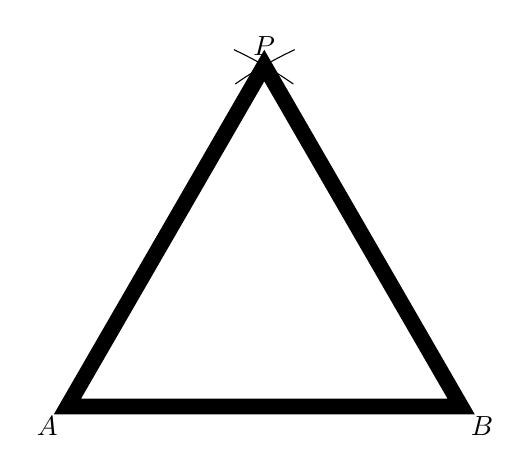
\begin{tikzpicture}

\coordinate (A) at (0, 0); % 定义点A
\coordinate (B) at (5, 0); % 定义点B
\draw[name path=A1] (A)+(55:5) arc(55:65:5); % 画圆弧A1,A为圆心,55-65度,半径5
\draw[name path=A2] (B)+(125:5) arc(125:115:5); % 画圆弧A2,B为圆心,125-115度,半径5
\path [name intersections={of=A1 and A2, by=P}]; % 求交点P
\draw[line width=0.2cm] (A) -- (B) -- (P) -- cycle; % 画连接A, B, P的三角形
\node at (A) [below left] {$A$}; % 标注点A
\node at (B) [below right] {$B$}; % 标注点B
\node at (P) [above] {$P$}; % 标注点P

\end{tikzpicture}
\end{document}
